\documentclass{beamer}
\usepackage[T1]{fontenc}
\usepackage[utf8]{inputenc}
\usepackage{listingsutf8}
\usepackage{listings}
% ---- IMPOSTAZIONI PACCHETTI ----
\definecolor{forestgreen}{rgb}{0.13, 0.55, 0.13}

\lstset{
    language=[LaTeX]Tex,%C++,
    keywordstyle=\color{blue}, %\bfseries,
    basicstyle=\small\ttfamily,
    commentstyle=\color{forestgreen}\ttfamily,
    stringstyle=\rmfamily,
    numbers=left,%
    numberstyle=\scriptsize, %\tiny
    stepnumber=1,
    numbersep=8pt,
    showstringspaces=false,
    breaklines=true,
    frameround=ftff,
    frame=single,
    inputencoding=utf8/latin1
}   
\usepackage{../UnipdTheme/Padova/beamerthemePadova}
\usepackage[absolute,overlay]{textpos}

\title{Package, theme e template}
\subtitle{Ovvero come rendere il documento più bello con il lavoro d'altri}
\author{Davide Polonio, Marco Zanella \& Emanuele Carraro}
\date{AA 2017-2018}


\begin{document}

	\maketitle
	\begin{frame}{Package}

\begin{itemize}
\item I \emph{package} possono essere visti come delle raccolte di funzionalità a cui possiamo accedere durante la scrittura di un documento

\vfill

\item Per usare un package il comando è 
\texttt{\textbackslash{}usepackage\{nome\_package\}}

\vfill

\item I package permettono di inserire immagini, cambiare il colore del testo,
inserire URL\dots{}

\end{itemize}

\end{frame}
	\begin{frame}[fragile]{Esempio}

\begin{exampleblock}{Senza l'utilizzo di package}
	\lstinputlisting{res/examples/withoututf8}
\end{exampleblock}

\pause

\begin{exampleblock}{Con l'utilizzo di package}
	\lstinputlisting{res/examples/withutf8}
\end{exampleblock}

\end{frame}

	\begin{frame}{Template}

\begin{itemize}
\item I \emph{template} invece possiamo pensarli come delle raccolte di comandi
che definiscono l'aspetto e i comandi per un certo documento
\item Possono definire anche i pacchetti utilizzati
\item Non definiremo mai un template ma molti sono disponibili online
\item Vediamo un esempio di template per la tesi!
\end{itemize}

\begin{figure}
	\centering
	
\includegraphics[scale=0.20]{res/images/template}
\end{figure}

\end{frame}

	\begin{frame}{Theme}

\begin{figure}
	\centering
	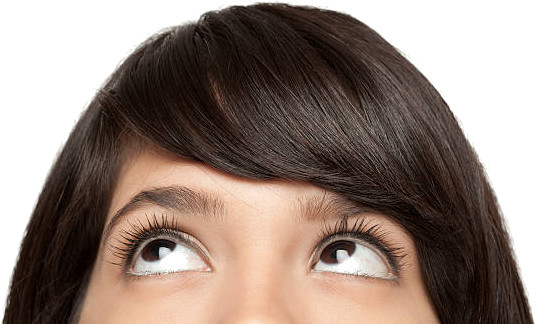
\includegraphics[scale=0.20]{res/images/temi}
\end{figure}

\begin{itemize}
	\item Si parla di temi invece nel caso di presentazioni \texttt{beamer}
	\item Anche in questo caso è possibile definirne uno proprio ma non lo
	faremo
	\item È possibile applicare un tema usando il comando
	\texttt{\textbackslash{}usetheme\{nome\_pacchetto\}}
	\item Certi temi permettono di scegliere la gamma di colori sfruttando il
	comando \texttt{\textbackslash{}usecolortheme\{nome\_colore\}}
\end{itemize}

\end{frame}

\end{document}
